\begin{figure}
\centering
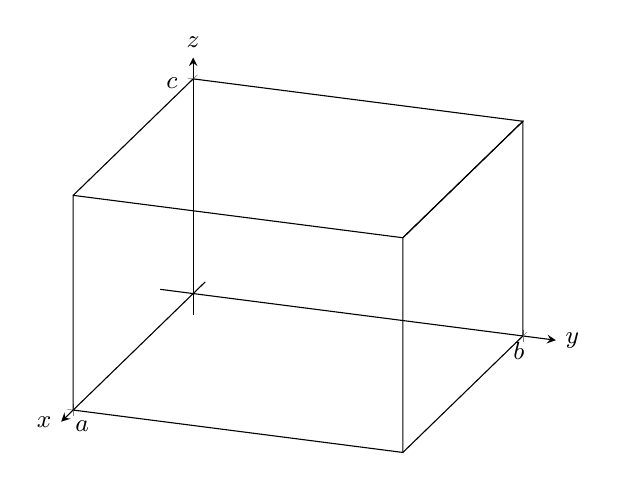
\begin{tikzpicture}[font=\small,]
\pgfmathsetmacro{\a}{1.5}
\pgfmathsetmacro{\b}{2}
\pgfmathsetmacro{\c}{1}
\begin{axis}[clip=false,axis lines=center,view/h=110,enlargelimits=true,xtick={\a},ytick={\b},ztick={\c},xticklabels={$a$},yticklabels={$b$},zticklabels={$c$},xlabel={$x$},ylabel={$y$},zlabel={$z$},xlabel style={anchor=east},ylabel style={anchor=west},zlabel style={anchor=south}]
\addplot3[]coordinates{(\a,0,0)(\a,\b,0)(\a,\b,\c)(\a,0,\c)(\a,0,0)};
\addplot3[]coordinates{(\a,\b,0)(0,\b,0)(0,\b,\c)(\a,\b,\c)};
\addplot3[]coordinates{(\a,0,\c)(0,0,\c)(0,\b,\c)(\a,\b,\c)};
\end{axis}
\end{tikzpicture}
\end{figure}

\begin{figure}
\centering
\begin{tikzpicture}[font=\small,]
\pgfmathsetmacro{\a}{1.5}
\pgfmathsetmacro{\b}{2}
\pgfmathsetmacro{\c}{1}
\begin{axis}[clip=false,axis lines=center,view/h=110,enlargelimits=true,xtick={\a},ytick={\b},ztick={\c},xticklabels={$a$},yticklabels={$b$},zticklabels={$c$},xlabel={$x$},ylabel={$y$},zlabel={$z$},xlabel style={anchor=east},ylabel style={anchor=west},zlabel style={anchor=south}, hide axis]
\addplot3[]coordinates{(1/2*\a,-1/3*\b,-1/3*\c)(1/2*\a,2/3*\b,-1/3*\c)(1/2*\a,-1/3*\b,2/3*\c)(1/2*\a,-1/3*\b,-1/3*\c)};
\addplot3[]coordinates{(1/2*\a,2/3*\b,-1/3*\c)(-1/2*\a,2/3*\b,-1/3*\c)(-1/2*\a,-1/3*\b,2/3*\c)(1/2*\a,-1/3*\b,2/3*\c)};
\addplot3[-latex]coordinates{(1/2*\a,0,0)(1.75*\a,0,0)}node[below]{$x$};
\addplot3[-latex]coordinates{(0,1/3*\b,0)(0,\b,0)}node[right]{$y$};
\addplot3[-latex]coordinates{(0,0,1/3*\c)(0,0,\c)}node[above]{$z$};
\addplot3[stealth-stealth]coordinates{(1/2*\a,0,-1/3*\c)(1/2*\a,0,0)}node[pos=0.5,right]{$\tfrac{c}{3}$};
\addplot3[stealth-stealth]coordinates{(1/2*\a,0,0)(1/2*\a,-1/3*\b,0)}node[pos=0.5,above]{$\tfrac{b}{3}$};
\addplot3[stealth-stealth]coordinates{(0,0,1/3*\c)(1/2*\a,0,1/3*\c)}node[pos=0.5,above left]{$\tfrac{a}{2}$};
\addplot3[]coordinates{(1/2*\a,1/3*\b,-1/3*\c)}node[below]{$b$};
\addplot3[]coordinates{(0,2/3*\b,-1/3*\c)}node[right]{$a$};
\addplot3[]coordinates{(1/2*\a,-1/3*\b,1/3*\c)}node[left]{$c$};
\addplot3[]coordinates{(-1/2*\a,1/3*\b,1/3*\c)}node[above,align=center]{\text{\RL{وسطانی مرکز}}\\  \عددی{(0,0,0)}};
\end{axis}
\end{tikzpicture}
\end{figure}


\begin{figure}
\centering
\begin{tikzpicture}[font=\small,declare function={fx(\r,\t)=2*\r*cos(\t);fy(\r,\t)=\r*sin(\t);fz(\r,\t)=2-2*\r*cos(\t);}]
\pgfmathsetmacro{\ta}{160}
\begin{axis}[clip=false,axis lines=center,view/h=160,enlargelimits=true,xlabel={$x$},ylabel={$y$},zlabel={$z$},xlabel style={anchor=east},ylabel style={anchor=west},zlabel style={anchor=south},xtick={\empty},ytick={\empty},ztick={\empty},hide axis]
\addplot3[smooth,domain y=0:360,variable y=\t] ({fx(1,t)},{fy(1,t)},{fz(1,t)})node[pos=0.75,pin=135:{$z=2-x$}]{};
\addplot3[smooth,domain y=0:360,variable y=\t] ({fx(1,t)},{fy(1,t)},0)node[pos=0.4,pin=-45:{$x^2+4y^2=4$}]{};
\addplot3[]coordinates{({fx(1,\ta)},{fy(1,\ta)},{fz(1,\ta)}) ({fx(1,\ta)},{fy(1,\ta)},0)};
\addplot3[dashed]coordinates{(0,0,0)(2,0,0)}node[circ]{}node[below]{$2$};
\addplot3[-latex]coordinates{(2,0,0)(2.5,0,0)}node[left]{$x$};
\addplot3[dashed]coordinates{(0,0,0)(0,1,0)}node[circ]{}node[below]{$1$};
\addplot3[-latex]coordinates{(0,1,0)(0,2,0)}node[right]{$y$};
\addplot3[dashed]coordinates{(0,0,0)(0,0,2)}node[circ]{}node[left]{$2$};
\addplot3[-latex]coordinates{(0,0,2)(0,0,4.5)}node[left]{$z$};
\end{axis}
\end{tikzpicture}
\end{figure}


\begin{figure}
\centering
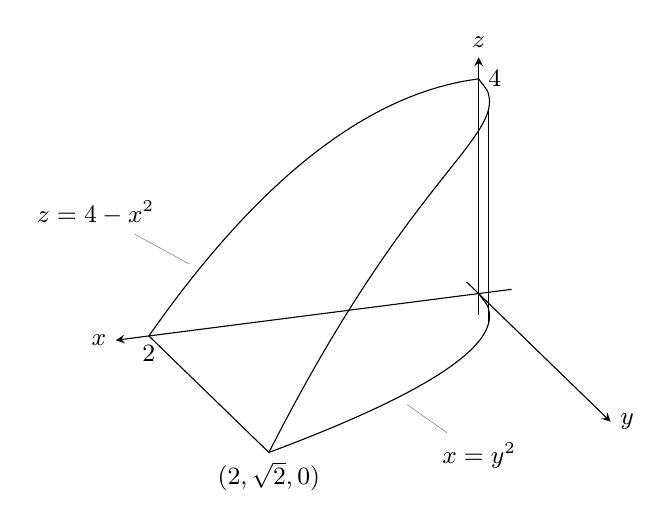
\begin{tikzpicture}[font=\small,declare function={fx(\x)=\x;fy(\x)=sqrt(\x);fz(\x)=4-(\x)^2;}]
\pgfmathsetmacro{\xa}{0.4}
\pgfmathsetmacro{\xb}{0.1}
\begin{axis}[clip=false,axis lines=center,view/h=160,enlargelimits=true,xlabel={$x$},ylabel={$y$},zlabel={$z$},xlabel style={anchor=east},ylabel style={anchor=west},zlabel style={anchor=south},xtick={\empty},ytick={\empty},ztick={\empty}]
\addplot3[smooth,domain=0:\xa,samples y=0] ({fx(x)},{fy(x)},{fz(x)});
\addplot3[smooth,domain=0:\xa,samples y=0] ({fx(x)},{fy(x)},0);
\addplot3[smooth,domain=\xa:2,samples y=0] ({fx(x)},{fy(x)},{fz(x)});
\addplot3[smooth,domain=\xa:2,samples y=0] ({fx(x)},{fy(x)},0)node[pos=0.4,pin=-45:{$x=y^2$}]{};
\addplot3[smooth,domain=0:2,samples y=0] ({fx(x)},0,{fz(x)})node[pos=0.75,pin=135:{$z=4-x^2$}]{};
\addplot3[]coordinates{(2,0,0)(2,sqrt(2),0)}node[pos=0,below]{$2$}node[below]{$(2,\sqrt{2},0)$};
\addplot3[]coordinates{ ({fx(\xb)},{fy(\xb)},{fz(\xb)}) ({fx(\xb)},{fy(\xb)},0)};
\addplot3[]coordinates{(0,0,4)}node[right]{$4$};
\end{axis}
\end{tikzpicture}
\end{figure}

\begin{figure}
\centering
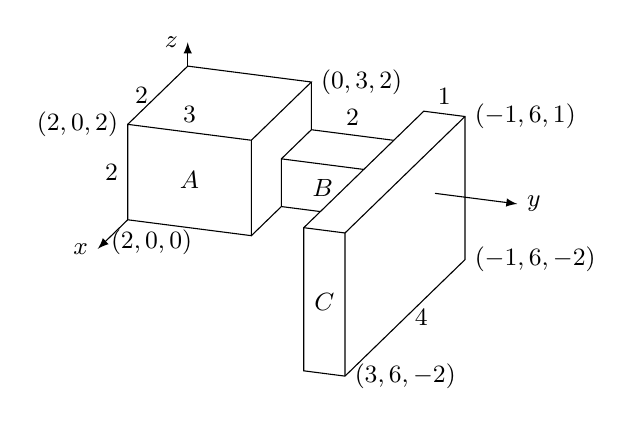
\begin{tikzpicture}[font=\small,declare function={fx(\x)=\x;fy(\x)=sqrt(\x);fz(\x)=4-(\x)^2;}]
\pgfmathsetmacro{\xa}{0.4}
\pgfmathsetmacro{\xb}{0.1}
\begin{axis}[clip=false,axis lines=center,view/h=110,enlargelimits=true,xlabel={$x$},ylabel={$y$},zlabel={$z$},xlabel style={anchor=east},ylabel style={anchor=west},zlabel style={anchor=south},xtick={\empty},ytick={\empty},ztick={\empty},hide axis]
\addplot3[]coordinates{(2,0,0)(2,3,0)(2,3,2)(2,0,2)(2,0,0)};
\addplot3[]coordinates{(2,3,2)(0,3,2)(0,0,2)(2,0,2)};
\addplot3[]coordinates{(2,3,0) (1,3,0) (1,3,1)(0,3,1) (0,3,2)};
\addplot3[]coordinates{(1,3,0)(1,5,0)};
\addplot3[]coordinates{(1,3,1)(1,5,1)};
\addplot3[]coordinates{(0,3,1)(0,5,1)};
\addplot3[fill=white]coordinates{(3,6,-2)(-1,6,-2)(-1,6,1)(-1,5,1)(3,5,1)(3,5,-2)(3,6,-2)};
\addplot3[]coordinates{(3,6,-2)(3,6,1)(-1,6,1)};
\addplot3[]coordinates{(3,5,1)(3,6,1)};
\addplot3[-latex]coordinates{(2,0,0)(3,0,0)}node[left]{$x$};
\addplot3[-latex]coordinates{(0,6,0)(0,8,0)}node[right]{$y$};
\addplot3[-latex]coordinates{(0,0,2)(0,0,2.5)}node[left]{$z$};
\addplot3[]coordinates{(2,0,2)}node[left]{$(2,0,2)$};
\addplot3[]coordinates{(2,0,0)}node[below,xshift=2ex]{$(2,0,0)$};
\addplot3[]coordinates{(3,6,-2)}node[right]{$(3,6,-2)$};
\addplot3[]coordinates{(-1,6,-2)}node[right]{$(-1,6,-2)$};
\addplot3[]coordinates{(-1,6,1)}node[right]{$(-1,6,1)$};
\addplot3[]coordinates{(0,3,2)}node[right]{$(0,3,2)$};
\addplot3[]coordinates{(-1,5.5,1)}node[above]{$1$};
\addplot3[]coordinates{(0,4,1)}node[above]{$2$};
\addplot3[]coordinates{(1,0,2)}node[left]{$2$};
\addplot3[]coordinates{(2,1.5,2)}node[above]{$3$};
\addplot3[]coordinates{(2,0,1)}node[left]{$2$};
\addplot3[]coordinates{(1,6,-2)}node[right]{$4$};
\addplot3[]coordinates{(2,1.5,1)}node[]{$A$};
\addplot3[]coordinates{(1,4,0.5)}node[]{$B$};
\addplot3[]coordinates{(3,5.5,-0.5)}node[]{$C$};
\end{axis}
\end{tikzpicture}
\end{figure}




\begin{figure}
\centering
\begin{tikzpicture}[font=\small,declare function={fx(\x)=cos(\x);fy(\x)=sin(\x);}]
\pgfmathsetmacro{\xa}{135}
\pgfmathsetmacro{\xb}{\xa+180}
\pgfmathsetmacro{\xc}{65}
\pgfmathsetmacro{\xd}{\xc+180}
\pgfmathsetmacro{\a}{1.5}
\pgfmathsetmacro{\b}{1.25}
\begin{axis}[clip=false,axis lines=center,view/h=135,enlargelimits=true,xlabel={$x$},ylabel={$y$},zlabel={$z$},xlabel style={anchor=east},ylabel style={anchor=west},zlabel style={anchor=south},xtick={\empty},ytick={\empty},ztick={\empty},hide  axis]
\addplot3[domain=0:360]({fx(x)},{fy(x)},2);
\addplot3[domain=0:360]({fx(x)},{fy(x)},0);
\addplot3[]coordinates{({fx(\xa)},{fy(\xa)},{2})({fx(\xa)},{fy(\xa)},0)};
\addplot3[]coordinates{({fx(\xb)},{fy(\xb)},{2})({fx(\xb)},{fy(\xb)},0)};
\addplot3[]coordinates{(-\a,-\b,2)(\a,-\b,2)(\a,\b,2)(-\a,\b,2)(-\a,-\b,2)};
\addplot3[]coordinates{({2*fx(\xc)},{2*fy(\xc)},2)({2*fx(\xc)},{2*fy(\xc)},0)({2*fx(\xd)},{2*fy(\xd)},0)({2*fx(\xd)},{2*fy(\xd)},2) ({2*fx(\xc)},{2*fy(\xc)},2)};
\addplot3[thick]coordinates{({fx(\xc)},{fy(\xc)},0)({fx(\xc)},{fy(\xc)},2)}node[circ]{}node[pin={[pin distance=1cm,right]-10:{$(\rho,\phi,z)$}}]{};
\addplot3[-stealth,domain=0:\xc,samples y=0] ({1.2*fx(x)},{1.2*fy(x)},0)node[pos=0.4,below]{$\phi$};
\addplot3[thick]coordinates{(0,0,0)({fx(\xc)},{fy(\xc)},0)}node[pos=0.6,left]{$\rho$};
\addplot3[dashed]coordinates{(0,0,0)(0,0,2)}node[circ]{}node[right]{$z$};
\addplot3[-latex]coordinates{(0,0,2)(0,0,3.5)}node[left]{$z$};
\addplot3[-latex]coordinates{(0,0,0)(2,0,0)}node[left]{$x$};
\addplot3[-latex]coordinates{(0,0,0)(0,2,0)}node[right]{$y$};
\end{axis}
\end{tikzpicture}
\end{figure}


\begin{figure}
\centering
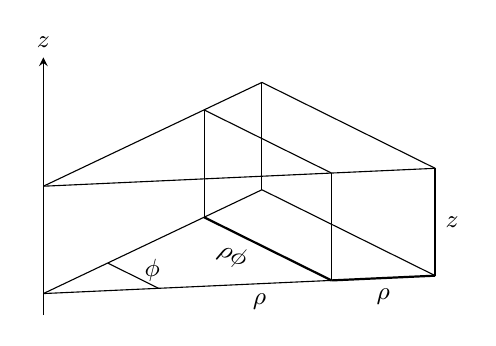
\begin{tikzpicture}[font=\small,declare function={fx(\r,\t)=\r*cos(\t);fy(\r,\t)=\r*sin(\t);}]
\pgfmathsetmacro{\ta}{30}
\pgfmathsetmacro{\tb}{\ta+45}
\pgfmathsetmacro{\ra}{1.25}
\pgfmathsetmacro{\rb}{\ra+0.45}
\pgfmathsetmacro{\h}{0.5}
\begin{axis}[clip=false,axis lines=center,view/h=20,enlargelimits=true,xlabel={$x$},ylabel={$y$},zlabel={$z$},xlabel style={anchor=east},ylabel style={anchor=west},zlabel style={anchor=south},xtick={\empty},ytick={\empty},ztick={\empty},xmin=0,ymin=0,zmin=0,zmax=1,hide x axis, hide y axis]
\addplot3[thick,domain y=\ta:\tb,samples=0,variable=\r,variable y=\t] ({fx(\ra,t)},{fy(\ra,t)},0)node[pos=0.7,sloped,below]{$\rho\dif\phi$};
\addplot3[domain y=\ta:\tb,samples=0,variable=\r,variable y=\t] ({fx(\rb,t)},{fy(\rb,t)},0);
\addplot3[domain y=\ta:\tb,samples=0,variable=\r,variable y=\t] ({fx(\ra,t)},{fy(\ra,t)},\h);
\addplot3[domain y=\ta:\tb,samples=0,variable=\r,variable y=\t] ({fx(\rb,t)},{fy(\rb,t)},\h);
\addplot3[thick]coordinates{({fx(\ra,\ta)},{fy(\ra,\ta)},0)({fx(\rb,\ta)},{fy(\rb,\ta)},0)}node[pos=0.5,below]{$\dif\rho$};
\addplot3[]coordinates{({fx(\ra,\tb)},{fy(\ra,\tb)},0)({fx(\rb,\tb)},{fy(\rb,\tb)},0)};
\addplot3[]coordinates{({fx(\ra,\ta)},{fy(\ra,\ta)},\h)({fx(\rb,\ta)},{fy(\rb,\ta)},\h)};
\addplot3[]coordinates{({fx(\ra,\tb)},{fy(\ra,\tb)},\h)({fx(\rb,\tb)},{fy(\rb,\tb)},\h)};
\addplot3[]coordinates{({fx(\ra,\ta)},{fy(\ra,\ta)},0)({fx(\ra,\ta)},{fy(\ra,\ta)},\h)};
\addplot3[thick]coordinates{({fx(\rb,\ta)},{fy(\rb,\ta)},0)({fx(\rb,\ta)},{fy(\rb,\ta)},\h)}node[pos=0.5,right]{$\dif z$};
\addplot3[]coordinates{({fx(\ra,\tb)},{fy(\ra,\tb)},0)({fx(\ra,\tb)},{fy(\ra,\tb)},\h)};
\addplot3[]coordinates{({fx(\rb,\tb)},{fy(\rb,\tb)},0)({fx(\rb,\tb)},{fy(\rb,\tb)},\h)};
\addplot3[]coordinates{(0,0,0)({fx(\ra,\ta)},{fy(\ra,\ta)},0)}node[pos=0.75,below]{$\rho$};
\addplot3[]coordinates{(0,0,0)({fx(\ra,\tb)},{fy(\ra,\tb)},0)};
\addplot3[]coordinates{(0,0,\h)({fx(\ra,\ta)},{fy(\ra,\ta)},\h)};
\addplot3[]coordinates{(0,0,\h)({fx(\ra,\tb)},{fy(\ra,\tb)},\h)};
\addplot3[samples=0,domain y=\ta:\tb,variable y=\t]({fx(0.5,t)},{fy(0.5,t)},0)node[pos=0.7,xshift=1ex,right]{$\dif \phi$};
\end{axis}
\end{tikzpicture}
\end{figure}



